%  LaTeX support: latex@mdpi.com
%  In case you need support, please attach all files that are necessary for compiling as well as the log file, and specify the details of your LaTeX setup (which operating system and LaTeX version / tools you are using).

%=================================================================
\documentclass[water,article,submit,moreauthors,pdftex]{mdpi}

% If you would like to post an early version of this manuscript as a preprint, you may use preprint as the journal and change 'submit' to 'accept'. The document class line would be, e.g., \documentclass[preprints,article,accept,moreauthors,pdftex]{mdpi}. This is especially recommended for submission to arXiv, where line numbers should be removed before posting. For preprints.org, the editorial staff will make this change immediately prior to posting.

%% Some pieces required from the pandoc template
\setlist[itemize]{leftmargin=*,labelsep=5.8mm}
\setlist[enumerate]{leftmargin=*,labelsep=4.9mm}


%--------------------
% Class Options:
%--------------------
%----------
% journal
%----------
% Choose between the following MDPI journals:
% acoustics, actuators, addictions, admsci, aerospace, agriculture, agriengineering, agronomy, algorithms, animals, antibiotics, antibodies, antioxidants, applsci, arts, asc, asi, atmosphere, atoms, axioms, batteries, bdcc, behavsci , beverages, bioengineering, biology, biomedicines, biomimetics, biomolecules, biosensors, brainsci , buildings, cancers, carbon , catalysts, cells, ceramics, challenges, chemengineering, chemistry, chemosensors, children, cleantechnol, climate, clockssleep, cmd, coatings, colloids, computation, computers, condensedmatter, cosmetics, cryptography, crystals, dairy, data, dentistry, designs , diagnostics, diseases, diversity, drones, econometrics, economies, education, electrochem, electronics, energies, entropy, environments, epigenomes, est, fermentation, fibers, fire, fishes, fluids, foods, forecasting, forests, fractalfract, futureinternet, futurephys, galaxies, games, gastrointestdisord, gels, genealogy, genes, geohazards, geosciences, geriatrics, hazardousmatters, healthcare, heritage, highthroughput, horticulturae, humanities, hydrology, ijerph, ijfs, ijgi, ijms, ijns, ijtpp, informatics, information, infrastructures, inorganics, insects, instruments, inventions, iot, j, jcdd, jcm, jcp, jcs, jdb, jfb, jfmk, jimaging, jintelligence, jlpea, jmmp, jmse, jnt, jof, joitmc, jpm, jrfm, jsan, land, languages, laws, life, literature, logistics, lubricants, machines, magnetochemistry, make, marinedrugs, materials, mathematics, mca, medicina, medicines, medsci, membranes, metabolites, metals, microarrays, micromachines, microorganisms, minerals, modelling, molbank, molecules, mps, mti, nanomaterials, ncrna, neuroglia, nitrogen, notspecified, nutrients, ohbm, particles, pathogens, pharmaceuticals, pharmaceutics, pharmacy, philosophies, photonics, physics, plants, plasma, polymers, polysaccharides, preprints , proceedings, processes, proteomes, psych, publications, quantumrep, quaternary, qubs, reactions, recycling, religions, remotesensing, reports, resources, risks, robotics, safety, sci, scipharm, sensors, separations, sexes, signals, sinusitis, smartcities, sna, societies, socsci, soilsystems, sports, standards, stats, surfaces, surgeries, sustainability, symmetry, systems, technologies, test, toxics, toxins, tropicalmed, universe, urbansci, vaccines, vehicles, vetsci, vibration, viruses, vision, water, wem, wevj

%---------
% article
%---------
% The default type of manuscript is "article", but can be replaced by:
% abstract, addendum, article, benchmark, book, bookreview, briefreport, casereport, changes, comment, commentary, communication, conceptpaper, conferenceproceedings, correction, conferencereport, expressionofconcern, extendedabstract, meetingreport, creative, datadescriptor, discussion, editorial, essay, erratum, hypothesis, interestingimages, letter, meetingreport, newbookreceived, obituary, opinion, projectreport, reply, retraction, review, perspective, protocol, shortnote, supfile, technicalnote, viewpoint
% supfile = supplementary materials

%----------
% submit
%----------
% The class option "submit" will be changed to "accept" by the Editorial Office when the paper is accepted. This will only make changes to the frontpage (e.g., the logo of the journal will get visible), the headings, and the copyright information. Also, line numbering will be removed. Journal info and pagination for accepted papers will also be assigned by the Editorial Office.

%------------------
% moreauthors
%------------------
% If there is only one author the class option oneauthor should be used. Otherwise use the class option moreauthors.

%---------
% pdftex
%---------
% The option pdftex is for use with pdfLaTeX. If eps figures are used, remove the option pdftex and use LaTeX and dvi2pdf.

%=================================================================
\firstpage{1}
\makeatletter
\setcounter{page}{\@firstpage}
\makeatother
\pubvolume{xx}
\issuenum{1}
\articlenumber{5}
\pubyear{2019}
\copyrightyear{2019}
%\externaleditor{Academic Editor: name}
\history{Received: date; Accepted: date; Published: date}
\updates{yes} % If there is an update available, un-comment this line

%% MDPI internal command: uncomment if new journal that already uses continuous page numbers
%\continuouspages{yes}

%------------------------------------------------------------------
% The following line should be uncommented if the LaTeX file is uploaded to arXiv.org
%\pdfoutput=1

%=================================================================
% Add packages and commands here. The following packages are loaded in our class file: fontenc, calc, indentfirst, fancyhdr, graphicx, lastpage, ifthen, lineno, float, amsmath, setspace, enumitem, mathpazo, booktabs, titlesec, etoolbox, amsthm, hyphenat, natbib, hyperref, footmisc, geometry, caption, url, mdframed, tabto, soul, multirow, microtype, tikz

%=================================================================
%% Please use the following mathematics environments: Theorem, Lemma, Corollary, Proposition, Characterization, Property, Problem, Example, ExamplesandDefinitions, Hypothesis, Remark, Definition
%% For proofs, please use the proof environment (the amsthm package is loaded by the MDPI class).

%=================================================================
% Full title of the paper (Capitalized)
\Title{Does the COMPAS Needle Always Point Towards Equity? Finding
Fairness in the COMPAS Risk Assessment Algorithm: A Case Study}

% Authors, for the paper (add full first names)
\Author{Amrita Acharya$^{1}$, Dianne Caravela$^{1}$, Eunice
Kim$^{1}$, Emma Kornberg$^{1}$, Elisabeth Nesmith$^{1}$}

% Authors, for metadata in PDF
\AuthorNames{Amrita Acharya, Dianne Caravela, Eunice Kim, Emma
Kornberg, Elisabeth Nesmith}

% Affiliations / Addresses (Add [1] after \address if there is only one affiliation.)
\address{%
$^{1}$ \quad Statistical and Data Sciences Smith College Northampton, MA
01063; \href{mailto:bbaumer@smith.edu}{\nolinkurl{bbaumer@smith.edu}}\\
}
% Contact information of the corresponding author
\corres{Correspondence: \href{mailto:aacharya@smith.edu}{\nolinkurl{aacharya@smith.edu}},
\href{mailto:dcaravela@smith.edu}{\nolinkurl{dcaravela@smith.edu}},
\href{mailto:ekim89@smith.edu}{\nolinkurl{ekim89@smith.edu}},
\href{mailto:ekornberg@smith.edu}{\nolinkurl{ekornberg@smith.edu}},
\href{mailto:enesmith@smith.edu}{\nolinkurl{enesmith@smith.edu}}}

% Current address and/or shared authorship








% The commands \thirdnote{} till \eighthnote{} are available for further notes

% Simple summary

% Abstract (Do not insert blank lines, i.e. \\)
\abstract{A variety of disciplines use risk assessment instruments to
help humans make data-driven decisions. Northpointe, a software company,
created an algorithmic risk assessment instrument known as the
Correctional Offender Management Profiling for Alternative Sanctions
(COMPAS). COMPAS uses various behavioral and psychological metrics
related to recidivism to assist justice systems in assessing a
defendant's potential recidivism risk. \citet{angwin2016machine}
published a ProPublica article in which they conclude that the racial
biases in the criminal justice system are reflected in the COMPAS
recidivism risk scores. In response, \citet{equivant_response_2016}
published a rebuttal on behalf of Northpointe defending the COMPAS
algorithm and refuting \citet{angwin2016machine}'s allegation of racial
bias. Using a human rights framework adopted from the organizations
Women at the Table and AI Fairness 360, we use debiasing algorithms and
fairness metrics to analyze the argument between Northpointe and
ProPublica and determine whether and to what extent there is racial bias
in the COMPAS algorithm.}

% Keywords

% The fields PACS, MSC, and JEL may be left empty or commented out if not applicable
%\PACS{J0101}
%\MSC{}
%\JEL{}

%%%%%%%%%%%%%%%%%%%%%%%%%%%%%%%%%%%%%%%%%%
% Only for the journal Diversity
%\LSID{\url{http://}}

%%%%%%%%%%%%%%%%%%%%%%%%%%%%%%%%%%%%%%%%%%
% Only for the journal Applied Sciences:
%\featuredapplication{Authors are encouraged to provide a concise description of the specific application or a potential application of the work. This section is not mandatory.}
%%%%%%%%%%%%%%%%%%%%%%%%%%%%%%%%%%%%%%%%%%

%%%%%%%%%%%%%%%%%%%%%%%%%%%%%%%%%%%%%%%%%%
% Only for the journal Data:
%\dataset{DOI number or link to the deposited data set in cases where the data set is published or set to be published separately. If the data set is submitted and will be published as a supplement to this paper in the journal Data, this field will be filled by the editors of the journal. In this case, please make sure to submit the data set as a supplement when entering your manuscript into our manuscript editorial system.}

%\datasetlicense{license under which the data set is made available (CC0, CC-BY, CC-BY-SA, CC-BY-NC, etc.)}

%%%%%%%%%%%%%%%%%%%%%%%%%%%%%%%%%%%%%%%%%%
% Only for the journal Toxins
%\keycontribution{The breakthroughs or highlights of the manuscript. Authors can write one or two sentences to describe the most important part of the paper.}

%\setcounter{secnumdepth}{4}
%%%%%%%%%%%%%%%%%%%%%%%%%%%%%%%%%%%%%%%%%%


% tightlist command for lists without linebreak
\providecommand{\tightlist}{%
  \setlength{\itemsep}{0pt}\setlength{\parskip}{0pt}}

% From pandoc table feature
\usepackage{longtable,booktabs,array}
\usepackage{calc} % for calculating minipage widths
% Correct order of tables after \paragraph or \subparagraph
\usepackage{etoolbox}
\makeatletter
\patchcmd\longtable{\par}{\if@noskipsec\mbox{}\fi\par}{}{}
\makeatother
% Allow footnotes in longtable head/foot
\IfFileExists{footnotehyper.sty}{\usepackage{footnotehyper}}{\usepackage{footnote}}
\makesavenoteenv{longtable}



\begin{document}


%%%%%%%%%%%%%%%%%%%%%%%%%%%%%%%%%%%%%%%%%%

\hypertarget{introduction}{%
\section{Introduction}\label{introduction}}

The Correctional Offender Management Profiling for Alternative Sanctions
(COMPAS) algorithm was created by the private, for-profit company
Northpointe (now known by its parent company
\href{https://www.equivant.com/faq/}{equivant}), to predict defendants'
risk of recidivism. It generates a decile score that classifies
defendants' risk of recidivism as either low, medium, or high
\citep{angwin2016machine}. Jurisdictions across the United States use
the COMPAS risk assessment instrument, including but not limited to the
\href{https://doccs.ny.gov/system/files/documents/2020/11/8500.pdf}{New
York},
\href{https://hdsr.mitpress.mit.edu/pub/hzwo7ax4/release/4}{Massachusetts},
\href{https://hdsr.mitpress.mit.edu/pub/hzwo7ax4/release/4}{Michigan},
\href{https://hdsr.mitpress.mit.edu/pub/hzwo7ax4/release/4}{California},
and \href{https://doc.wi.gov/Pages/AboutDOC/COMPAS.aspx}{Wisconsin}
Departments of Corrections.

Due to the proprietary nature of the COMPAS algorithm, it is unknown how
exactly these recidivism risk scores are calculated; however, a
\href{https://www.documentcloud.org/documents/2702103-Sample-Risk-Assessment-COMPAS-CORE\#document/p5/a296598}{sample
COMPAS Risk Assessment Survey} has been made publicly available,
revealing the algorithm's input information. This survey has been widely
critiqued for using proxy variables for race that do not explicitly
factor in a defendant's race but heavily imply it, allowing Northpointe
to claim that their algorithm is free of racial bias. For example, the
COMPAS risk assessment survey asks screeners to speculate if a defendant
might be affiliated with a gang. It also asks if a defendant has any
friends or family members who have been crime victims
\citep{Angwin2016Sample}. Although these questions do not directly ask
about race, they do not take into account the pervasive nature of
systemic racism that infiltrates every aspect of the lives of
marginalized people, thereby indirectly asking about race.
\citet{angwin2016machine}. published a 2016 piece in the news
publication ProPublica that analyzes the methods and algorithms used by
Northpointe in their COMPAS risk score assessment algorithm and uncovers
the racial biases in defendants' scores \citep{angwin2016machine}. Their
research finds that ``the algorithm {[}is{]} somewhat more accurate than
a coin flip,'' a worrisome level of accuracy given the potential impact
its determinations may have on real people's lives.
\citet{angwin2016machine} specifically investigate the distribution of
COMPAS scores by decile among Black and white defendants. They write:
``The analysis also {[}shows{]} that even when controlling for prior
crimes, future recidivism, age, and gender, Black defendants {[}are{]}
45 percent more likely to be assigned higher risk scores than white
defendants'' \citep{larson2016we}. After examining the fairness metric
statistical parity difference, \citet{angwin2016machine} conclude that
the algorithm is racially biased \citep{larson2016we}.

\citet{equivant_response_2016}, on the behalf of Northpointe, deny the
allegations of racial bias and offer their own analyses based on
different fairness metrics in rebuttal \citep{equivant_response_2016}.
\citet{angwin2016machine} maintain that there are biases in the outcome
values, protected attributes, and covariates during
\citet{equivant_response_2016}'s data processing phase. ProPublica
collaborators \citet{larson2016we} account for these biases in their
analyses. In their response, \citet{equivant_response_2016} highlight
that \citet{angwin2016machine} did not account for base rates of
recidivism in their analysis, which are important to understand initial
percentages without the presence of other information.

\href{https://www.womenatthetable.net/}{Women at the Table}, the sponsor
organization for this project, is ``a growing, global gender equality \&
democracy CSO based in Geneva, Switzerland focused on advancing feminist
systems change by using the prism of technology, innovation \& AI
exercising leverage points in technology, the economy, sustainability \&
democratic governance.'' We are collaborating with the organization on
its AI \& Equality \citep{noauthor_ai_nodate} initiative, tasked with
de-biasing the COMPAS algorithm \citep{aif360-oct-2018} and producing a
corresponding data story that will be added to its library.

Our project builds on Women at the Table's various de-biasing algorithms
used in its AI \& Equality Human Rights Toolbox to conduct our own
analyses on the COMPAS data set. Based on this analysis, we employ a
human rights framework to contribute to the ProPublica and Northpointe
debate and investigate whether or to what extent there is racial bias in
the COMPAS algorithm. With a solid understanding of the two sides, we
aim to pinpoint the shortcomings of both arguments and correct them in
our analyses. We will use various de-biasing techniques and fairness
metrics to evaluate the level of bias present in the COMPAS data and our
algorithm. We will summarize our results using the JupyterNotebook
framework from Women at the Table, to be used by members of the
organization to teach in a workshop setting. We hope that our findings
will highlight the importance of checking statistical analyses using
varied methods and contribute to the ongoing discussion of the effects
of machine biases in the justice system.

\hypertarget{data}{%
\section{Data}\label{data}}

The data we are using for this project is the COMPAS General Recidivism
Risk Scores data set from the AI Fairness 360 (AIF360) toolkit
\citep{aif360-oct-2018}, which does the same initial pre-processing as
ProPublica. The raw data has 6,167 rows and each row represents an
arrest charge for a defendant. AIF360's COMPAS data includes the
defendant's age, race, sex, prior charges, what they were charged with,
and whether or not the defendant ultimately recidivated within a
two-year period after their arrest. For the purposes of our project,
which endeavors to evaluate the differing effects of the COMPAS
algorithm on white defendants versus Black defendants, we have filtered
the data to only include individuals whose race is listed as Caucasian
or African-American. Our data therefore has 5,723 rows (Figure
\ref{fig:table snip}), with the below distributions of race (Figure
\ref{fig:race plot}), age (Figure \ref{fig:age plot}), and two year
recidivism rate (Figures \ref{fig:recid plot} \&
\ref{fig:recid race plot} and Table \ref{tab:recid table}).

\begin{figure}

{\centering 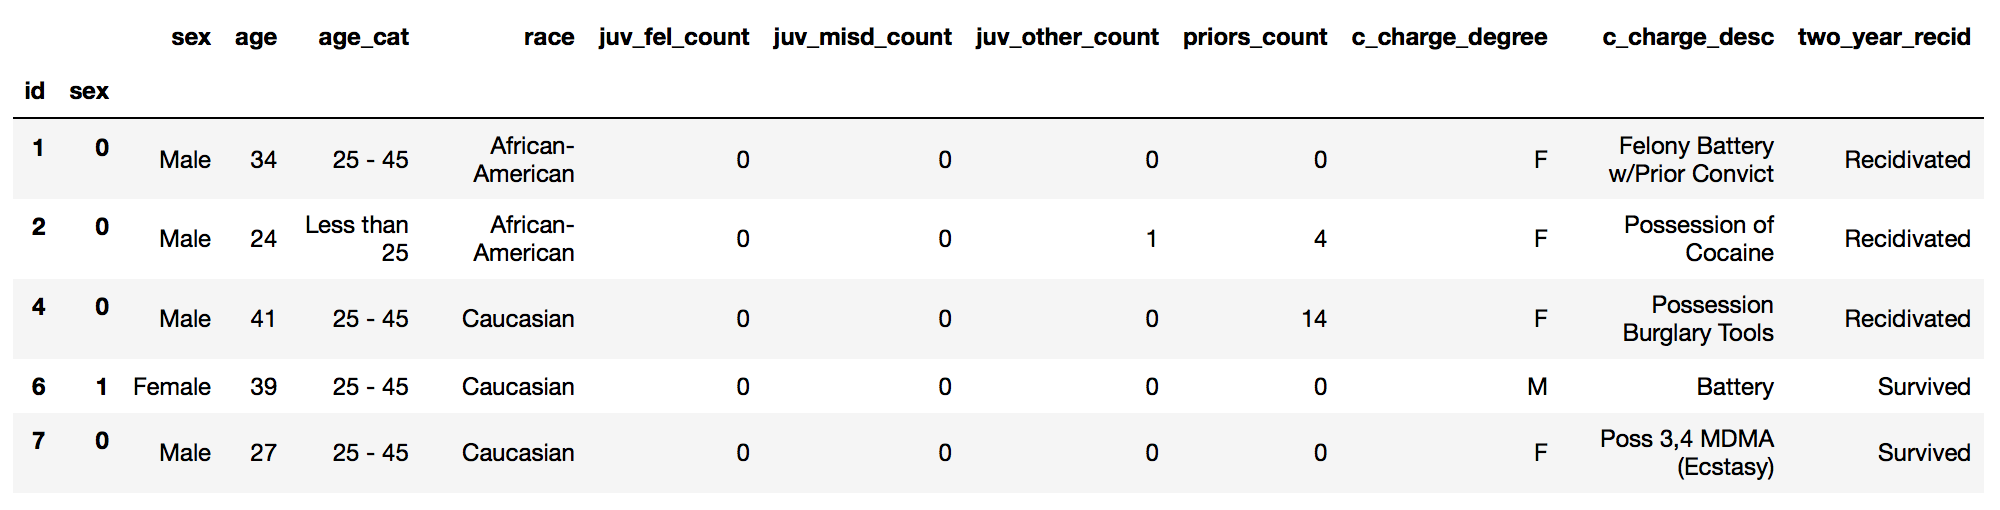
\includegraphics[width=1\linewidth]{../images/table_snippet} 

}

\caption{This table is a snippet of the data set we will be using, containing information on a defendant's age, sex, race, criminal history, charge degree, charge description, and two year recidivism outcome.}\label{fig:table snip}
\end{figure}

\begin{figure}

{\centering 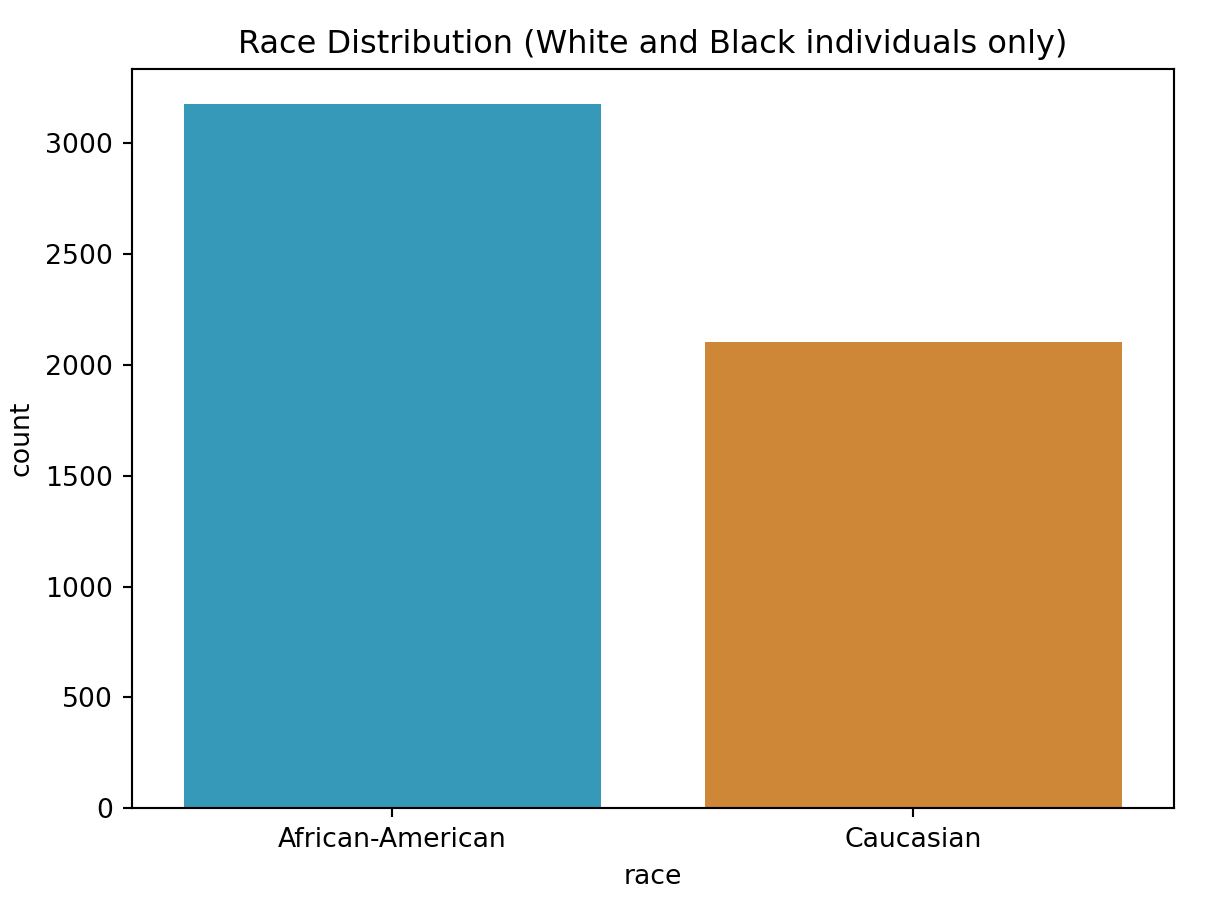
\includegraphics[width=1\linewidth]{../images/race_bar_plot_new} 

}

\caption{This plot shows the distribution of defendant races. The dataset contains about 3200 Black defendants and 2100 white defendants. Therefore, there are more Black people represented in the dataset than white people.}\label{fig:race plot}
\end{figure}

\begin{figure}

{\centering 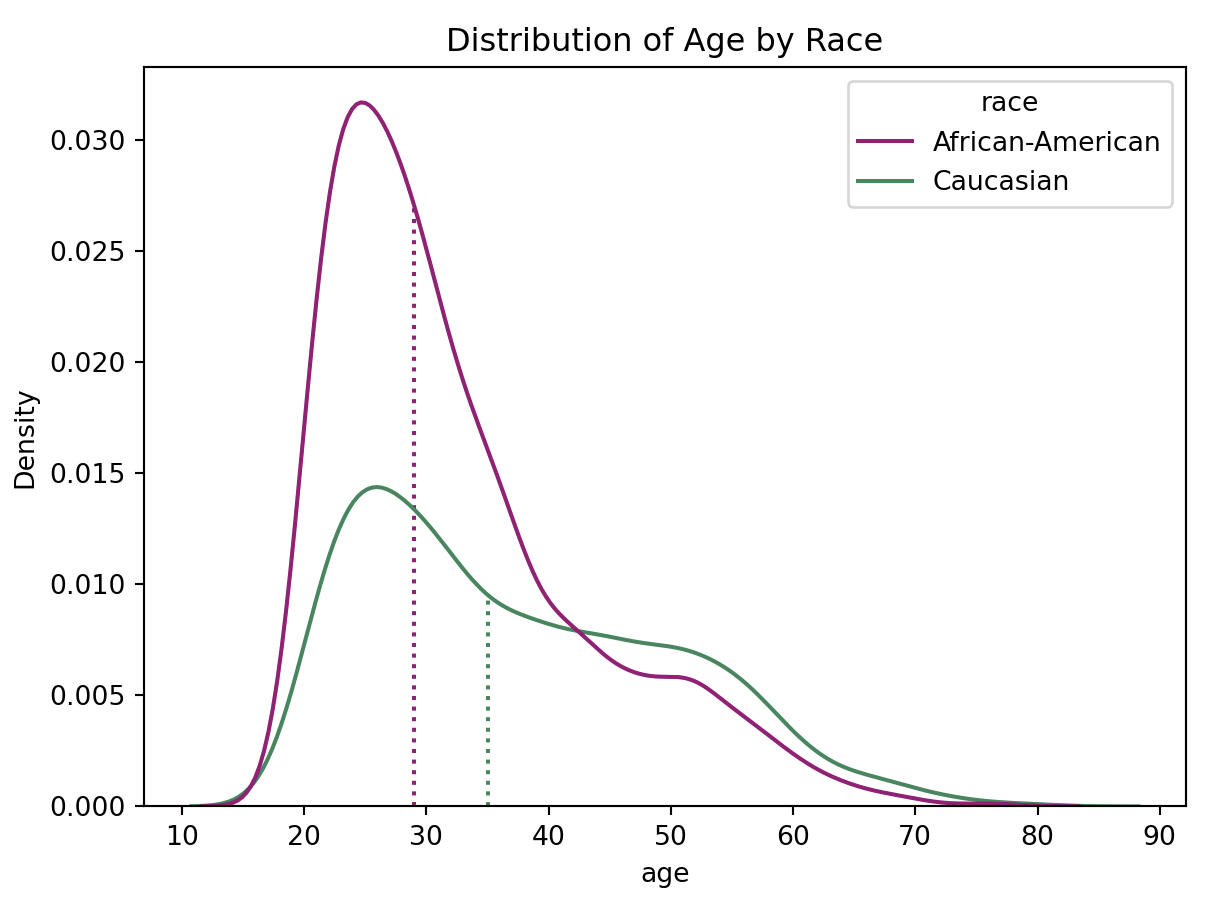
\includegraphics[width=1\linewidth]{../images/age_race_plot_new} 

}

\caption{This plot shows the distribution of defendant ages by race. The purple curve shows the distribution of the ages of Black defendants, and the green curve shows the distribution of the ages of white defendants. The probability of a defendant's age being between two points on the x-axis is the total shaded area of the curve under the two points. The purple dotted line represents the median age of Black defendants (29 years) and the green dotted line represents the median age of white defendants (35 years). For both groups, the majority of defendants are relatively young, but this is especially noticeable for Black defendants.}\label{fig:age plot}
\end{figure}

\begin{figure}

{\centering 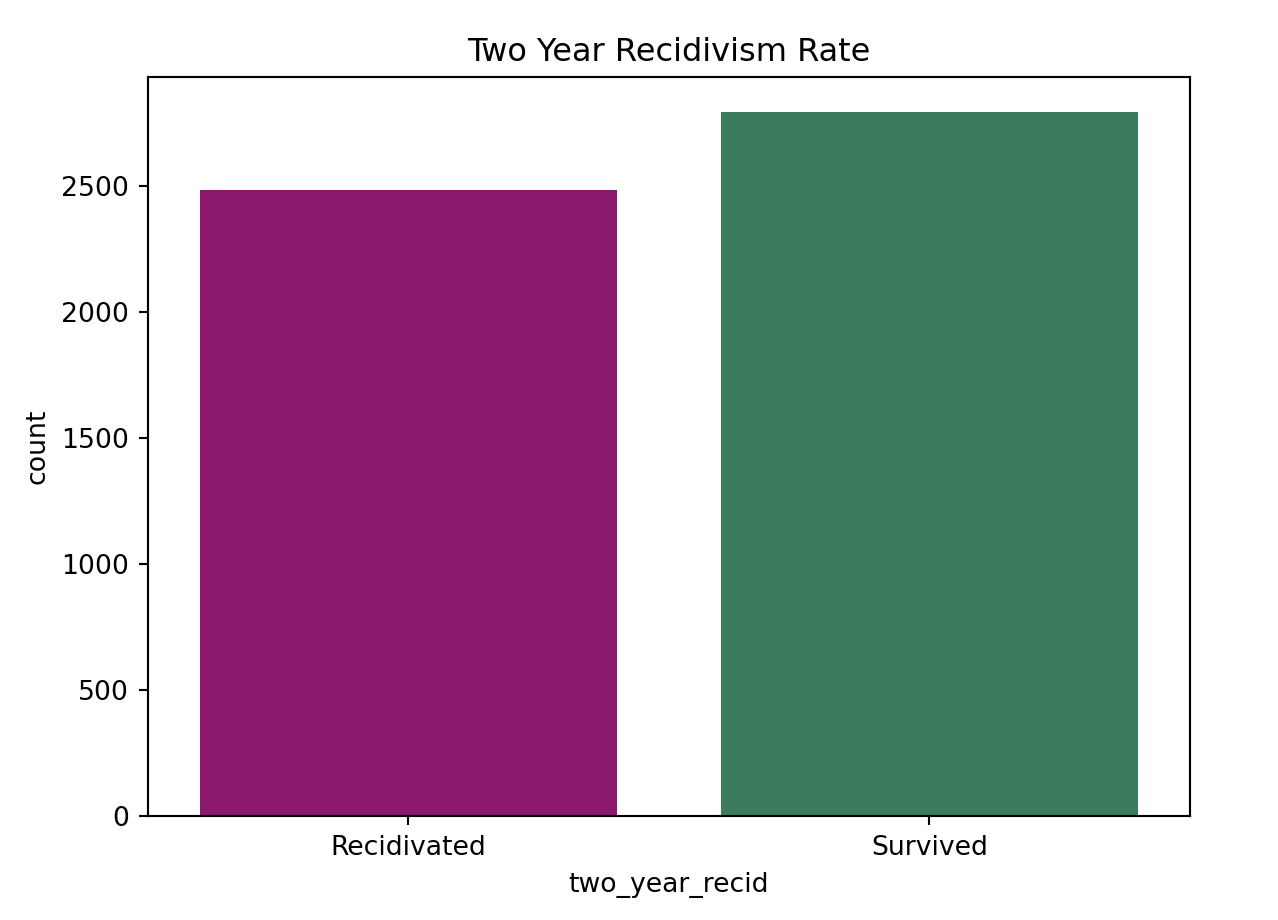
\includegraphics[width=1\linewidth]{../images/recid_bar_plot_new} 

}

\caption{This plot shows the distribution of two year recidivism outcomes. Out of all defendants, there is a higher proportion of people who did not recidivate than who did. About 2500 people recidivated, whereas approximately 2700 did not.}\label{fig:recid plot}
\end{figure}

\begin{figure}

{\centering 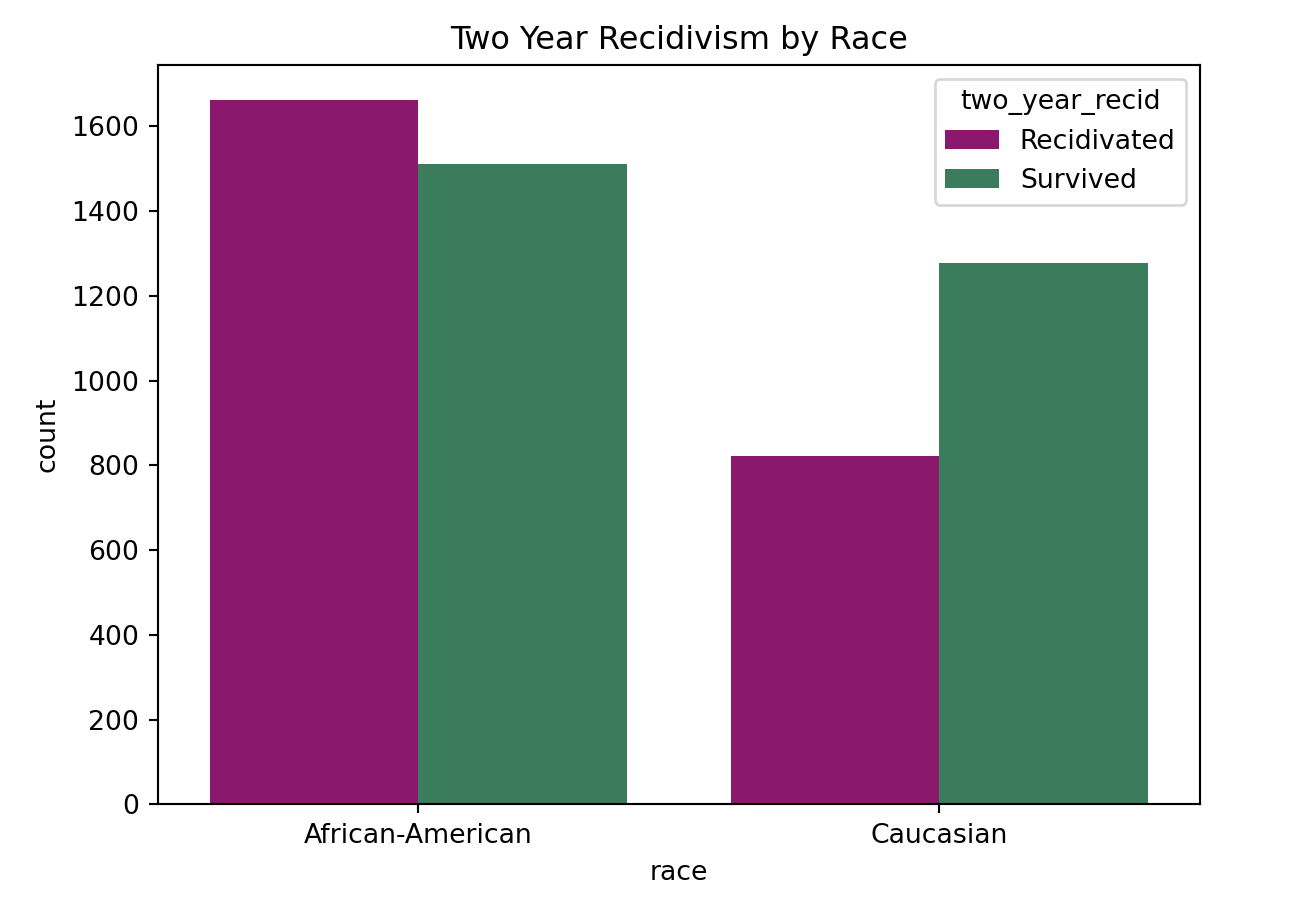
\includegraphics[width=1\linewidth]{../images/race_recid_bar_plot_new} 

}

\caption{This plot shows the distribution of two year recidivism outcomes by race. When we divide the data into Black and white defendants, we can see that Black defendants recidivate more than white defendants and Black defendants are more likely to recidivate than not recidivate. We can also see that there are more Black defendants in the dataset overall.}\label{fig:recid race plot}
\end{figure}

\begin{longtable}[]{@{}lll@{}}
\caption{This table shows the counts of recidivism by race, illustrating
how a much greater proportion (\textgreater{} 50\%) of Black defendants
recidivated than their white counterparts.
\label{tab:recid table}}\tabularnewline
\toprule
Two Year Recidivism by Race & Recidivated & Survived \\
\midrule
\endfirsthead
\toprule
Two Year Recidivism by Race & Recidivated & Survived \\
\midrule
\endhead
African American & 1661 & 1512 \\
Caucasian & 822 & 1278 \\
\bottomrule
\end{longtable}

\hypertarget{methods}{%
\section{Methods}\label{methods}}

AI Fairness 360 (AIF360) is an open-source Python toolkit that seeks to
``to help facilitate the transition of fairness research algorithms to
use in an industrial setting and to provide a common framework for
fairness researchers to share and evaluate algorithms''
\citep{aif360-oct-2018}. It contains multiple data sets, including the
COMPAS data set that accompanied the \citet{angwin2016machine} piece.

The AIF360 toolkit contains various group and individual fairness
metrics as well as pre-processing, in-processing, and post-processing
algorithms that we used for our experiments \citep{aif360-oct-2018}. We
researched the definitions and applications of different fairness
metrics \citep{ashokan2021fairness} to determine which metric would be
most appropriate for our project. We chose to look at four group
fairness metrics instead of individual fairness metrics. Group fairness
takes into account the attributes of a whole group as opposed to just
one individual in the group, allowing us to represent more of the
systemic issues happening. In general, group fairness metrics require
that the unprivileged group is treated similarly to the privileged
group, whereas individual fairness metrics require individuals to be
treated consistently \citep{kypraiou_what_2021}. Group and individual
metrics work in opposition of one another, meaning that when group
fairness improves, individual fairness gets worse.

\textbf{Statistical Parity Difference} - This metric measures the
difference that the majority and protected classes get a particular
outcome. The ideal value of this metric is 0. Fairness for this metric
is between -0.1 and 0.1. A negative value means there is higher benefit
for the privileged group (in this case, white defendants).

\[P(\hat{Y}=1|D=Unprivileged) - P(\hat{Y}=1|D=Privileged)\]

\textbf{Disparate Impact Ratio} - This metric is the ratio of how often
the favorable outcome occurs in one group versus the other. In the case
of recidivism, this is the ratio of how many white defendants are
predicted to not recidivate compared to how many Black defendants are
predicted to not recidivate. A value of 1 means that the ratio is
exactly 1:1. Less than 1 means the privileged group (white defendants)
benefits, while a value greater than 1 means the unprivileged group
(Black defendants) benefits. According to AIF360, a ratio between .8 to
1.25 is considered fair\citep{Ronaghan2019AI}.

\[\frac{P(\hat{Y}=1|D=Unprivileged)}{P(\hat{Y}=1|D=Privileged)}\]

\textbf{Average Odds Difference} - This metric returns the average
difference in false positive rate and true positive rate for the
privileged and unprivileged groups. A value of 0 indicates equality of
odds, and a value below 0 implies benefit for the privileged group.
Equality of odds is achieved in the case of recidivism when the
proportion of people who were predicted to recidivate and did recidivate
is equal (true positive rate) for both Black and white defendants AND
the proportion of people who were predicted to recidivate and did not
recidivate (false positive rate) is equal for both Black and white
defendants\citep{aif360-oct-2018}.

\[\frac{(FPR_{D = unprivileged} - FPR_{D = privileged}) + (TPR_{D = unprivileged} - TPR_{D = privileged})}{2}\]

\textbf{Equal Opportunity Difference} - This metric is computed as the
difference of true positive rates between the unprivileged and the
privileged groups. The true positive rate is the ratio of true positives
to the total number of actual positives for a given
group\citep{GoogleDev}.

The ideal value is 0. A value less than 0 implies higher benefit for the
privileged group and a value greater than 0 implies higher benefit for
the unprivileged group. Fairness for this metric is between -0.1 and 0.1
\citep{aif360-oct-2018}.

This metric is best used when it is very important to catch positive
outcomes while false positives are not exceptionally problematic
\citep{Cortez2019How}. This is not the case for the COMPAS data set, as
false positives mean extra jail time for someone who will not actually
re-offend.

\[TPR_{D = Unprivileged} - TPR_{D = Privileged}\]

For the next step of our experiment, we need to determine where in the
data science pipeline we can mitigate the most bias, using
pre-processing, in-processing, and post-processing de-biasing
algorithms. These are all based on using predictive models to figure out
how we can ``fix'' the bias that is present.

Pre-processing refers to assessing the training data, and it is the most
flexible method because it has not yet trained a model that may carry
assumptions about the data. It is important to keep in mind that
pre-processing prevents assumptions in the modeling, but does not
account for the bias in data collection. With pre-processing, we use the
re-weighing algorithm from AIF360 which weights the examples in each
(group, label) combination differently to ensure fairness before
classification \citep{aif360-oct-2018}. We use a logistic regression
model for this algorithm, as it is the easiest to interpret in the given
context. After running the fairness metrics using the pre-processing
algorithm, we are able to compare our results to the baseline metrics
from the previous section.

Another approach, in-processing, explores how bias can be targeted while
building a model. It assesses how we build learning algorithms, which
often prioritize accuracy over fairness. The technique we use is the
Meta Classification algorithm, which accounts for the fairness metric as
part of the input and returns a classifier optimized by that particular
metric. Similarly to pre-processing, we compare the results of our
in-processing methods with both the baseline and the pre-processing to
gauge which method so far has better individual or group fairness.

Our last approach, post-processing, makes transformations on model
outputs. Similarly to the pre-processing, it is flexible because it does
not work directly with the algorithm, but instead has direct access to
all the predicted classification values. Because the algorithms are
often so complex and difficult to interpret, post-processors are trained
in a black box. To get around this, we use the PostProcessingMeta class
from AIF360 which combines the training and prediction for a random
estimator and the post-processor while simultaneously splitting the data
set \citep{aif360-oct-2018}. Based on these results, we look
comparatively at all the approaches to determine which we assess to be
the most fair.

\hypertarget{preliminary-results}{%
\section{Preliminary Results}\label{preliminary-results}}

With our baseline model, we ran the four different group fairness
metrics we chose and compared the results (pictured in Table
\ref{tab:baseline metrics table}))

The statistical parity difference is -0.14. This indicates that there is
a large difference between white and Black defendants regarding whether
or not they recidivate. The algorithm unfairly benefits white defendants
over Black defendants. Disparate impact ratio is 0.47. The ratio of
white defendants predicted to not recidivate to the Black defendants
predicted to not recidivate is 0.47. A ratio between 0.8 and 1.25 is
considered fair, therefore the algorithm unfairly benefits white
defendants.

Average odds difference is -0.44. The average difference in false
positive rates and true positive rates for white and Black defendants is
-0.44. Values less than zero are considered in favor of the privileged
group, so the algorithm unfairly benefits white defendants.

Equal opportunity difference is -0.41. The difference of true positive
rates between the Black and white groups is -0.41. A value less than 0
indicates a benefit to the privileged group, so the algorithm unfairly
benefits white defendants. The value is substantially less than -0.1,
which indicates that the algorithm benefits white defendants.

All four group fairness metrics determine that the COMPAS algorithm
favors white defendants over Black defendants. The statistical parity
metric indicates unfairness by a smaller margin of 0.04 than equal
opportunity difference which has a margin of error 0.4 below the
threshold. Although this is true, each algorithm uses different
penalties for unfavorable outcomes, so the higher the penalty the more
of a difference there will be between the fairness threshold and the
value.

\begin{longtable}[]{@{}llll@{}}
\caption{Results of Baseline Fairness Metric Analysis
\label{tab:baseline metrics table}}\tabularnewline
\toprule
Fairness Metric & Ideal Value & Baseline Value & Benefited Group \\
\midrule
\endfirsthead
\toprule
Fairness Metric & Ideal Value & Baseline Value & Benefited Group \\
\midrule
\endhead
Statistical Parity Difference & 0 & -0.14 & White Defendants \\
Disparate Impact Ratio & 1 & 0.47 & White Defendants \\
Average Odds Difference & 0 & -0.44 & White Defendants \\
Equal Opportunity Difference & 0 & -0.41 & White Defendants \\
\bottomrule
\end{longtable}

% %%%%%%%%%%%%%%%%%%%%%%%%%%%%%%%%%%%%%%%%%%
% %% optional
% \supplementary{The following are available online at www.mdpi.com/link, Figure S1: title, Table S1: title, Video S1: title.}
%
% % Only for the journal Methods and Protocols:
% % If you wish to submit a video article, please do so with any other supplementary material.
% % \supplementary{The following are available at www.mdpi.com/link: Figure S1: title, Table S1: title, Video S1: title. A supporting video article is available at doi: link.}

\vspace{6pt}

%%%%%%%%%%%%%%%%%%%%%%%%%%%%%%%%%%%%%%%%%%

%%%%%%%%%%%%%%%%%%%%%%%%%%%%%%%%%%%%%%%%%%

%%%%%%%%%%%%%%%%%%%%%%%%%%%%%%%%%%%%%%%%%%

%%%%%%%%%%%%%%%%%%%%%%%%%%%%%%%%%%%%%%%%%%
%% optional


%%%%%%%%%%%%%%%%%%%%%%%%%%%%%%%%%%%%%%%%%%
% Citations and References in Supplementary files are permitted provided that they also appear in the reference list here.

%=====================================
% References, variant A: internal bibliography
%=====================================
%\reftitle{References}
%\begin{thebibliography}{999}
% Reference 1
%\bibitem[Author1(year)]{ref-journal}
%Author1, T. The title of the cited article. {\em Journal Abbreviation} {\bf 2008}, {\em 10}, 142--149.
% Reference 2
%\bibitem[Author2(year)]{ref-book}
%Author2, L. The title of the cited contribution. In {\em The Book Title}; Editor1, F., Editor2, A., Eds.; Publishing House: City, Country, 2007; pp. 32--58.
%\end{thebibliography}

% The following MDPI journals use author-date citation: Arts, Econometrics, Economies, Genealogy, Humanities, IJFS, JRFM, Laws, Religions, Risks, Social Sciences. For those journals, please follow the formatting guidelines on http://www.mdpi.com/authors/references
% To cite two works by the same author: \citeauthor{ref-journal-1a} (\citeyear{ref-journal-1a}, \citeyear{ref-journal-1b}). This produces: Whittaker (1967, 1975)
% To cite two works by the same author with specific pages: \citeauthor{ref-journal-3a} (\citeyear{ref-journal-3a}, p. 328; \citeyear{ref-journal-3b}, p.475). This produces: Wong (1999, p. 328; 2000, p. 475)

%=====================================
% References, variant B: external bibliography
%=====================================
\reftitle{References}
\externalbibliography{yes}
\bibliography{mybibfile.bib}

%%%%%%%%%%%%%%%%%%%%%%%%%%%%%%%%%%%%%%%%%%
%% optional

%% for journal Sci
%\reviewreports{\\
%Reviewer 1 comments and authors’ response\\
%Reviewer 2 comments and authors’ response\\
%Reviewer 3 comments and authors’ response
%}

%%%%%%%%%%%%%%%%%%%%%%%%%%%%%%%%%%%%%%%%%%


\end{document}
